\subsection{Stochastic block model}
\label{sec:SBM}
In the previous section, we extended the \ER~random graph to the general configuration model to detect and quantify statistically significant variations in node degrees. In this section, we introduce the stochastic block model (SBM), which similarly models group structures such as those discussed in Section~\ref{sec:group-structure}.

Groups in networks are often characterized as communities of tightly connected nodes. In the examples shown in Figure~\ref{fig:community-examples}a-c, the groups are assortative as indicated by the high number of edges~$\mIn$ between nodes of the same group. To count these intra-group edges, we index the groups by~$r = 1,...,q$ and represent group assignments as an $n$-vector of integers~$\vec{b}$, where each node~$i$ belongs to group~$b_i \in \{1,...,q\}$. In this notation, the number of edges inside groups is \begin{align}
    \mIn = \frac{1}{2} \sum_{i,j=1}^n A_{ij} \delta_{b_ib_j},
\end{align}
where the Kronecker delta~$\delta_{b_ib_j}$ restricts the sum to nodes~$i$ and~$j$ in the same group. While a large number of edges~$\mIn$ within the groups suggests a strong group structure, it is important to contextualize this count. Even if there is no assortative preference, randomly placed edges can fall within groups and contribute to~$\mIn$. 

To establish a baseline for~$\mIn$, we use the microcanonical configuration model Eq.~\eqref{eq:P-A-given-k} as a null hypothesis. This generates alternative networks that match the observed node degrees but lack inherent group structure. Under this randomization, the expected number of edges between any two nodes~$i$ and~$j$ is \begin{align}
    \mathbf{E} A_{ij} = \frac{k_i k_j}{2m}.
\end{align}
We thus expect a total number of intra-group edges \begin{align}
    \langle \mIn \rangle_{\text{config}} &= \frac{1}{2}\sum_{ij} \frac{k_ik_j}{2m} \delta_{b_ib_j}.
\end{align}
To demonstrate that the groups are meaningfully assortative, we then check if the count~$\mIn$ observed in the network is surprising relative to this expectation.

A measure known as the \emph{modularity}~\cite{Newman06b} quantifies and normalizes this difference as \begin{align}
    Q(A,\vec{b}) &= \frac{1}{m}\left(\mIn - \langle \mIn \rangle_{\text{config}}\right) \nonumber \\
    &= \frac{1}{2m}\sum_{ij} \left(A_{ij} - \frac{k_ik_j}{2m}\right) \delta_{b_ib_j}. \label{eq:modularity}
\end{align}
This definition ensures that the expected modularity of a partition is 0, and a positive value indicates that the network is more assortative, or \emph{modular}, than we would expect.

Within the significance testing framework, we can also compute the p-value that the configuration model could generate a network as assortative as the observed case. Figure~\ref{fig:modularity-large} shows an example of this test on the network of Division IA college football matches considered in the previous section. Here we can calculate the modularity of the network across the~$q = 12$ conferences, represented by node colors in Figure~\ref{fig:modularity-large}a. Across the season, $\mIn = 397$ of the $m = 616$ matches are played between teams in the same conference (highlighted in green), leading to a network modularity of~$Q = 0.555$. Figure~\ref{fig:modularity-large}b compares the modularity along this partition in the real network to that in 10,000 alternative networks drawn from the configuration model. Across these cases the largest modularity obtained is~$Q = 0.041$, indicating that there is a very statistically significant preference for teams to play within their own conference. 

\begin{figure}
    \centering
    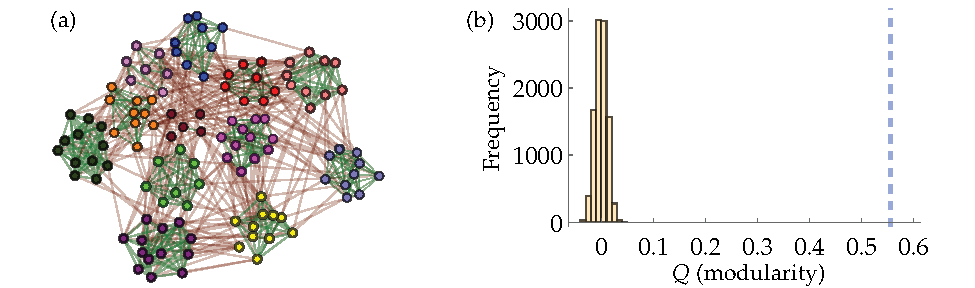
\includegraphics{max_dissertation//chapters//figures//chp1/modularity-large.pdf}
    \caption{(a) Football match network with edges within groups highlighted in green and edges between groups in red. (b) Modularity of the conference partition of the football match network (vertical dashed line) compared to 10,000 alternative networks with the same degree sequence sampled from the configuration model.}
    \label{fig:modularity-large}
\end{figure}

In an unsupervised setting, where the group structure of the network is unknown, the modularity is often used not only to measure behavior but also to identify groups. In this approach, a "good" group structure is defined as one with high modularity, where groups contain significantly more internal edges than expected by chance. Thus, for a given network~$\mat{A}$, the best-fit group structure is the optimum \begin{align}
    \vec{b}^* = \argmax_{\vec{b}} Q(\mat{A},\vec{b}),
\end{align}
where $\vec{b}^*$ is found using one of several \emph{modularity maximization} methods. Some commonly used algorithms are discussed in Appendix~\ref{app:algorithms}. 

Applying this strategy to the football match network, we can find a partition of the teams into 11 groups with modularity~$Q = 0.601$. Remarkably, this partition closely resembles the "true" conference group structure. Using the information-theoretic similarity measure defined in Chapter~\ref{chp:information}, the found partition scores a 0.865 out of 1. From the network alone, we can thus nearly recover the original conferences. Encouraged by this result, we can apply this method to help uncover groups of nodes that meaningfully influence the structure of the network, even when such groups are initially unknown. 

While this modularity maximization approach has been widely used to great effect in network science~\cite{Barber07, Boccaletti07, GDC10}, it has certain limitations. One major issue is overfitting. Consider a graph that inherently lacks a group structure, such as those generated by \ER~or configuration models. In such cases the appropriate "partition" of the nodes places them into one large group,~$\vec{b} = (1,...,1)$. From the definition of the modularity, this all-in-one grouping has~$Q = 0$ for any network~$\mat{A}$. However, when optimizing the modularity, it is typically possible to find some other partition of the nodes into more than one group that is at least slightly assortative,~$Q > 0$, merely due to random graph fluctuations. Modularity maximization will therefore prefer this over-fitted partition over the true single group. 

Figure~\ref{fig:modularity-small} exemplifies this issue by illustrating the network of matches played within only the Big Ten college football conference in 2022. This network presumably lacks group structure, given that it represents a single conference. Yet, the modularity is maximized at positive~$Q = 0.156$ by dividing the teams into two groups, as shown in Figure~\ref{fig:modularity-small}a. In Figure~\ref{fig:modularity-small}b we again consider this modularity in the context of 10,000 alternative networks that share the same degree sequence. In this case, the observed modularity is not clearly separated from what the configuration model predicts, but still yields a p-value $P = 0.01$. In isolation, this might imply a statistically significant assortative pattern. However, given that this grouping was selected among~$2^{n - 1} - 1 = 8191$ possible two-group partitions, is it not unexpected that one might exhibit such a low p-value. Since the modularity alone can never return a null result, modularity maximization must be combined with such significance testing that is often challenging to interpret. 

\begin{figure}
    \centering
    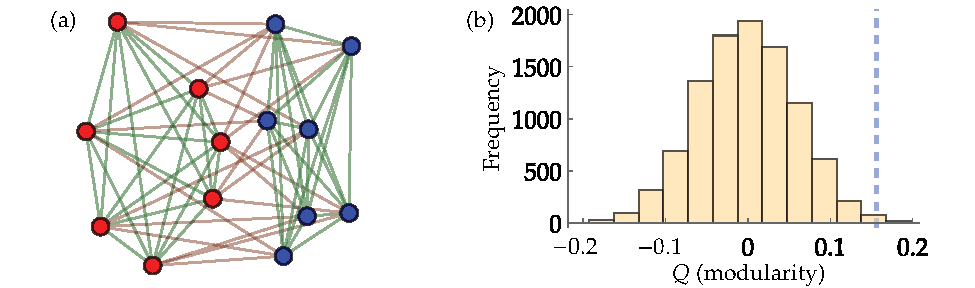
\includegraphics{max_dissertation//chapters//figures//chp1/modularity-small.pdf}
    \caption{(a) Network of football matches within only the Big Ten conference. The teams are partitioned into two groups to maximize modularity. (b) The modularity along the optimized partition compared that in 10,000 networks with the same degree sequence sampled from the configuration model.}
    \label{fig:modularity-small}
\end{figure}

Even when no true assortative pattern is present, modularity maximization will overfit and report some slightly assortative partition. In cases where the actual group structure is \emph{disassortative}, such as the bipartite network of Figure~\ref{fig:community-examples}d, modularity maximization will also fail to identify the true groups. This is because disassortative groups do not align with modularity's fundamentally assortative definition of a community. To successfully identify such groups, we must broaden our definition to include these cases, or even more complex structural patterns like mixtures of assortative and disassortative groups. 

The root of these issues lies in the fact that modularity maximization is not a generative model, unlike the \ER~or configuration models described earlier. While the partition that maximizes the modularity is useful for describing and summarizing assortative network structures, it does not provide a mechanism for their formation. This precludes us from employing our usual Bayesian inference tools to prevent overfitting or from using the modularity to make predictions. 

While some efforts have been made to directly convert the modularity objective function into a generative model~\cite{PK23}, in this thesis we instead consider \emph{stochastic block models} (SBMs). These models come in a variety of different flavors~\cite{KN11a, Peixoto14a, YL2020}, some of which we introduce in Chapter~\ref{chp:group-structure}. They provide the flexibility to model a wide range of possible group structures and can be directly compared against the other generative models we have considered.

The traditional stochastic block model is defined by the assumption that the probability two nodes~$i$ and $j$ are connected depends only on their group identities~$b_i$ and $b_j$. Some pairs of groups may be more likely to be connected than others, but all nodes within the same group share the same structural role: they are identically and independently likely to be connected to nodes in other groups. These probabilities across groups form a symmetric~$q \times q$ \emph{weight matrix}~$\mat{\omega}$, where~$\omega_{rs}$ is the expected number of edges between each node in group~$r$ and each node in group~$s$. This framework effectively defines what we mean by groups: node labels that influence the pattern of connections. This pattern can be quite generic as we do not assume the groups are defined by a globally assortative or disassortative preference.

For each pair of groups~$r$ and~$s$, the weight matrix entry~$\omega_{rs}$ plays the same role as the overall density~$\rho$ in the \ER~multigraph model Eq.~\eqref{eq:ER-multigraph-canonical}. Each edge count~$A_{ij}$ is modeled as a Poisson distribution with expectation~$\omega_{b_ib_j}$. Consequently, the usual SBM models the interior of each group~$r$ as a random multigraph with density~$\omega_{rr}$ and assumes connections between groups occur independently and identically. 

By building the model in this way, the SBM becomes a nested model that includes an \ER~random graph as the special case where all nodes are assigned to a single group,~$\vec{b} = (1,...,1)$. Just as the general configuration model, this nested structure allows us to directly compare the SBM against the \ER~model it extends. Collecting these assumptions, the likelihood that a network is generated by a group structure~$\vec{b}$ and weights~$\mat{\omega}$ in the SBM is then
\begin{align}
    P(\mat{A}|\mat{\omega},\vec{b}) &= \prod_{i < j}\frac{\omega_{b_ib_j}^{A_{ij}}e^{-\omega_{b_ib_j}}}{A_{ij}!}  \prod_{i=1}^n \frac{(\omega_{b_ib_i}/2)^{A_{ii}/2}e^{-\omega_{b_ib_i}/2}}{(A_{ii}/2)!}. \label{eq:P-A-given-omega-b}
\end{align}

We can condense this expression by introducing some useful notation. We denote the number of nodes in group~$r$ as \begin{align}
    n_r = \sum_{i=1}^n \delta_{b_ir},
\end{align}
forming the $q$-vector of integers~$\vec{n}$, and count the number of edges that run between groups~$r, s = 1,...,q$ as \begin{align}
    M_{rs} = \sum_{i,j=1}^n A_{ij} \delta_{b_ir}\delta_{b_js}, \label{eq:M-edge-count-matrix}
\end{align}
entries of the symmetric~$q \times q$ \emph{edge count matrix}~$\mat{M}$. Analogous to the adjacency matrix, the diagonal elements of this edge count matrix~$M_{rr}$ are twice the number of edges that run internally between nodes in group~$r$. This convention ensures that the row sum of the edge count matrix~$\vec{m}$ has entries 
\begin{align}
    m_r = \sum_{s = 1}^q M_{rs} = \sum_{i=1}^n k_i \delta_{b_ir}
\end{align}
equal to the total degree of the nodes in each group. With this notation we can then collect the likelihood terms as
\begin{align}
    P(\mat{A}|\mat{\omega},\vec{b}) &= \frac{1}{\prod_{i<j}A_{ij}!\prod_i A_{ii}!!} \prod_{r<s}\omega_{rs}^{M_{rs}} e^{-n_rn_s \omega_{rs}}\prod_{r=1}^q \omega_{rr}^{M_{rr}/2} e^{-n_r^2 \omega_{rr}/2}.
\end{align}

At this stage, we may be tempted to perform a maximum-likelihood estimate and find the choice of weights~$\mat{\omega}$ and partition~$\vec{b}$ most likely to produce the observed network. Unfortunately this approach has serious issues. Consider the group partition~$\vec{b} = (1,...,n)$ that places each node in its own group and the weight matrix~$\mat{\omega} = \mat{A}$ between the now~$n$ groups. Although this choice of parameters then has a very high model likelihood Eq.~\eqref{eq:P-A-given-omega-b}, as each edge~$A_{ij}$ is drawn from a Poisson distribution of the same mean~$A_{ij}$, the overall model is woefully over-parametrized. The weight matrix alone contains as many parameters as the data~$\mat{A}$ itself and overfits the network.

Our familiar solution to this problem is to carefully introduce priors over the parameters~$\mat{\omega}$ and~$\vec{b}$ that reflect what we expect "typical" weight and group structures to look like. As in the general configuration model, the choices of these priors matter considerably in realistic network applications. For example in Section~\ref{sec:assortative-SBM} we discuss how the choice of weight matrix prior~$P(\mat{\omega})$ drastically influences model behavior. In this introduction, however, we will review the choices most often made for the traditional SBM. 

Over possible group structures~$\vec{b}$ we use a prior
\begin{align}
    P(\vec{b}) &= P(\vec{b}|\vec{n})P(\vec{n}|q)P(q) \nonumber \\
    &= \frac{\prod_r n_r!}{n!} \binom{n-1}{q-1}^{-1}\frac{1}{n} \label{eq:P-b}
\end{align}
which is uniform over the number of groups~$q$ ranging from~$1$ to~$n$, over the possible node count vectors~$\vec{n}$ as positive integer vectors of length~$q$ that sum to~$n$, and over the possible partitions~$\vec{b}$ that satisfy the node counts~$\vec{n}$. This structure of the prior ensures that \textit{a priori} we have no preference for any particular number of communities~$q$. For instance there is prior probability~$P(q = 1) = 1/n$ that all nodes belong in one group. This case recovers the \ER~random graph, the possibility of no community structure. If we had instead used a prior that is simply uniform over all possible~$n$-vectors of integers from 1 to $n$, the prior would heavily weigh a large number of communities, as most such labelings have a number of distinct groups~$q \sim n$, and~$q = 1$ would be effectively excluded from the prior distribution.

For the weight matrix~$\mat{\omega}$, we traditionally use i.i.d. exponential priors of mean~$\rho > 0$ on the upper triangular entries~$\omega_{rs}$ where~$r \leq s$. To generate a symmetric matrix, we then set the entries below the diagonal to those above it as $\omega_{sr} = \omega_{rs}$. This gives the prior over symmetric weight matrices \begin{align}
    P(\mat{\omega}|\rho) = \prod_{r \leq s}\frac{1}{\rho} e^{-\omega_{rs}/\rho}. \label{eq:P-omega-given-rho}
\end{align} 
We call~$\rho$ the \emph{density} parameter here since it is equal to the expected network density averaged over both the likelihood and the weight matrix prior as \begin{align}
    \mathbf{E}\frac{2m}{n^2} = \frac{1}{n^2} \mathbf{E} \sum_{ij} A_{ij} = \frac{1}{n^2} \sum_{ij} \mathbf{E} \omega_{b_ib_j} = \rho.
\end{align}
If the number of edges~$m$ is known, this density parameter is often set to its empirical point estimate $\hat{\rho} = 2m/n^2$. However, in keeping with our fully Bayesian presentation we instead allow the parameter to run free with the same exponential prior used for the \ER~graph, $P(\rho) = e^{-\rho}$.

An example of this generative process is shown in Figure~\ref{fig:SBM-generation}. Although we start as in the \ER~model by setting the overall density~$\rho$, the entries of the weight matrix~$\mat{\omega}$ can then fluctuate from this expectation, producing a network structure differentiated by group. In this example the weight matrix generates an assortative group structure, although the choice of~$\mat{\omega}$ can specify an arbitrary pattern of connections. 

\begin{figure}
    \centering
    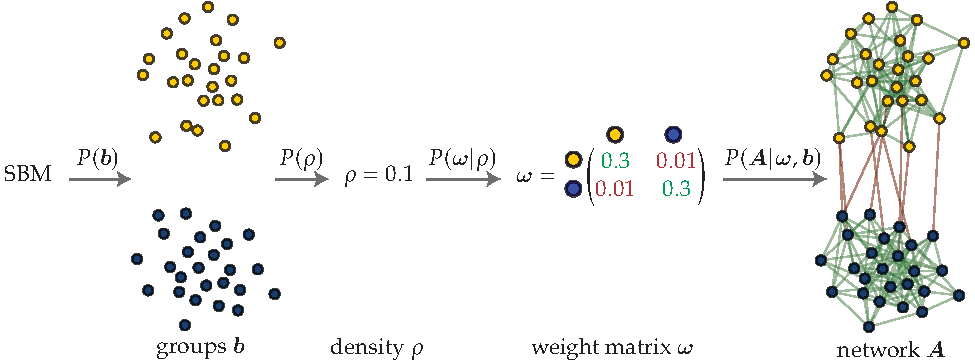
\includegraphics{max_dissertation//chapters//figures//chp1/SBM-generation.pdf}
    \caption{Example generative process for the stochastic block model of group structure. The group each node belongs to~$\vec{b}$, represented by the colors, is first sampled. The overall density~$\rho$ is then sampled and used to generate the symmetric weight matrix~$\omega$. In the final network~$\mat{A}$ the density of edges between a node in group~$r$ and a node in group~$s$ is given by the entry~$\omega_{rs}$. In this example the edges within groups (colored green) are much more likely than edges between groups (red), resulting in an assortative group structure.}
    \label{fig:SBM-generation}
\end{figure}

In many applications, we will mainly be interested in inferring the group structure~$\vec{b}$ of the network rather than the weight matrix. For this purpose we \emph{marginalize} over the possible weight matrices~$\mat{\omega}$ to obtain the integrated likelihood \begin{align}
    P(\mat{A}|\vec{b},\rho) &= \int P(\mat{A}|\mat{\omega},\vec{b})P(\mat{\omega}|\rho) d\mat{\omega} \nonumber \\
    &= \underbrace{\frac{\prod_{r < s} M_{rs}! \prod_r M_{rr}!!/n_r^{m_r}}{\prod_{i<j}A_{ij}!\prod_i A_{ii}!!}}_{\text{multinomial}} \> \underbrace{\prod_{r < s} \frac{(\rho n_r n_s)^{M_{rs}}}{(\rho n_r n_s + 1)^{M_{rs} + 1}}\prod_r \frac{(\rho n_r^2/2)^{M_{rr}/2}}{(\rho n_r^2/2 + 1)^{M_{rr}/2 + 1}}}_{\text{geometric}} \nonumber \\
    &= P(\mat{A}|\mat{M},\vec{b})P(\mat{M}|\vec{n},\rho). \label{eq:P-A-given-b-rho}
\end{align}
This expression again factorizes into a microcanonical picture. The edge count matrix entries are distributed geometrically, while the positions of the edges between groups are distributed multinomially. 

In terms of this integrated likelihood, we can use Bayes' law to write the posterior distribution over potential group structures and densities \begin{align}
    P(\vec{b},\rho|\mat{A}) = \frac{P(\mat{A}|\vec{b},\rho)P(\vec{b})P(\rho)}{P(\mat{A})}
\end{align}
This can be a complex multimodal distribution as many group structures are possible, although often only the maximum a posteriori (MAP) estimate of the community structure is reported as the best fit. For a more complete picture we can sample potential group structures from this posterior distribution using Markov Chain Monte Carlo (MCMC) methods detailed in Appendix~\ref{app:SBM-monte-carlo}. These sampled partitions can then be summarized in a number of ways~\cite{LF12, KN22}, including the consensus clustering method discussed in Appendix~\ref{app:consensus-clustering}.

In Figure~\ref{fig:SBM-posteriors} we show the results of this posterior sampling for the Division IA and Big Ten networks from earlier this section. We plot the posterior distributions of the number of found communities~$q$ for each network. Since a single community~$q = 1$ reduces to the \ER~random graph, its density in the posterior distribution reflects the relative evidence of the \ER~graph and the full SBM. The posteriors thus show that the Big Ten conference is best described by the \ER~model while the full Division IA network warrants the stochastic block model. From the peak of the posterior, we also observe that the SBM finds~$q = 10$ communities in the Division IA network, again slightly less than the 12 "true" conferences. These model selections are also confirmed by the cross-validation performances of the models on the data sets reported in Table~\ref{tab:SBM-performances}.

\begin{figure}
    \centering
    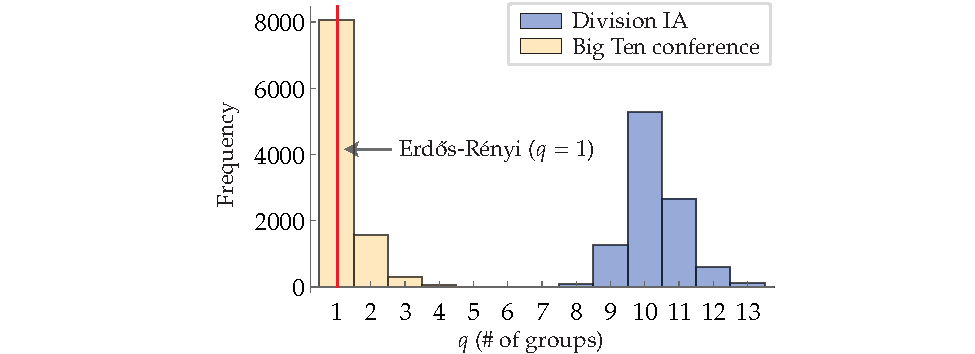
\includegraphics{max_dissertation//chapters//figures//chp1/SBM-posteriors.pdf}
    \caption{Posterior distributions of the number of groups~$q$ found by the stochastic block model within the networks of football matches within only the Big Ten conference (orange) and the entire Division IA (blue). The special case of~$q = 1$, for which the SBM reduced to the \ER~random graph is highlighted in red. We observe that while there is considerable evidence of group structure in the Division IA network, likely into 10 groups. The Big Ten conference, however, does not meaningfully have internal group structure.}
    \label{fig:SBM-posteriors}
\end{figure}

% 
\begin{table}[htbp]
\centering
\begin{tabular}{l||cc|cc}
Data set & \multicolumn{2}{c|}{Division IA}      & \multicolumn{2}{c}{Big Ten conference}             \\ \hline
Model        & \ER & SBM        & \ER & SBM \\ \hline
$\hat{q}_{\text{MAP}}$ & N/A & $10$ & N/A & $1$ \\ 
$H(\mat{A})$ & $4335.0$ & $\mathbf{3584.5}$ & $\mathbf{171.8}$ & $172.8$  \\ 
$H(\Atest|\Atrain)$ & $859.0$ & $\mathbf{710.5}$ & $\mathbf{33.89}$ & $34.03$
\end{tabular}
\caption{Table of the number of communities~$\hat{q}$ found by the SBM, the Bayesian evidence~$H(\mat{A})$, and posterior-predictive~$H(\Atest|\Atrain)$ for \ER~and stochastic block models on the Division IA and Big Ten conference football match networks.}
\label{tab:SBM-performances}
\end{table}

Although the stochastic block model thus offers a Bayesian framework for inferring and justifying community structures, the model still has certain limitations. For one, the model shares the same homogeneous distribution of degrees as the \ER~random model it is based upon. In order to create a model that captures both the group structure of the SBM and the degree variation of the configuration model we will need to \emph{degree-correct} the SBM as described in Section~\ref{sec:SBM-degree-correction}~\cite{KN11a}. There we will observe that different networks call for various amounts of this degree correction, just as the general configuration model encompasses a spectrum of degree variation. 

Secondly, the model suffers from a so-called \emph{resolution limit} where the model is unable to find communities smaller than a certain size, even when they are well-separated~\cite{FB07}. This drawback is shared with modularity maximization, as seen by both the SBM and modularity maximization finding fewer than the true~$q = 12$ communities of the football network. We discuss why this occurs and how to adjust the SBM to address this effect in Section~\ref{sec:assortative-SBM}.

More fundamentally, all stochastic block models, including the novel ones presented in this thesis cannot find communities beyond a \emph{detectability threshold} where the assortative (or disassortative) preference that defines the groups is too weak to recover among the noise~\cite{Abbe18}. In fact, this threshold is an inherent limitation of any method for identifying such groups. In Section~\ref{sec:reduced-mutual-information-paper} we will observe how a wide variety of community detection algorithms run into the same barrier. This threshold is analogous to the phase transition of the Ising model foundational to statistical physics, a perspective we discuss more in Appendix~\ref{app:SBM-Ising}~\cite{Moore17}. Although some sufficiently weak group structures can not be reliably inferred, this thesis introduces methods to uncover groups closer to this limit in Chapter~\ref{chp:group-structure}.